\documentclass[a4paper,12pt]{article}
\usepackage[utf8]{inputenc}
\usepackage[russian]{babel}
\usepackage{amsmath}
\usepackage{amssymb}
\usepackage{enumitem}
\usepackage{graphicx}
\usepackage{hyperref}
\usepackage[a4paper, top= 1cm, bottom=2cm, left=2cm, right=2cm]{geometry}

\hypersetup{
    colorlinks=true,
    linkcolor=blue,
    urlcolor=blue, 
}

\title{Кролики и клетки}

\begin{document}
\maketitle

\begin{figure}[h]
    \raggedleft
    \vspace{-5cm}
    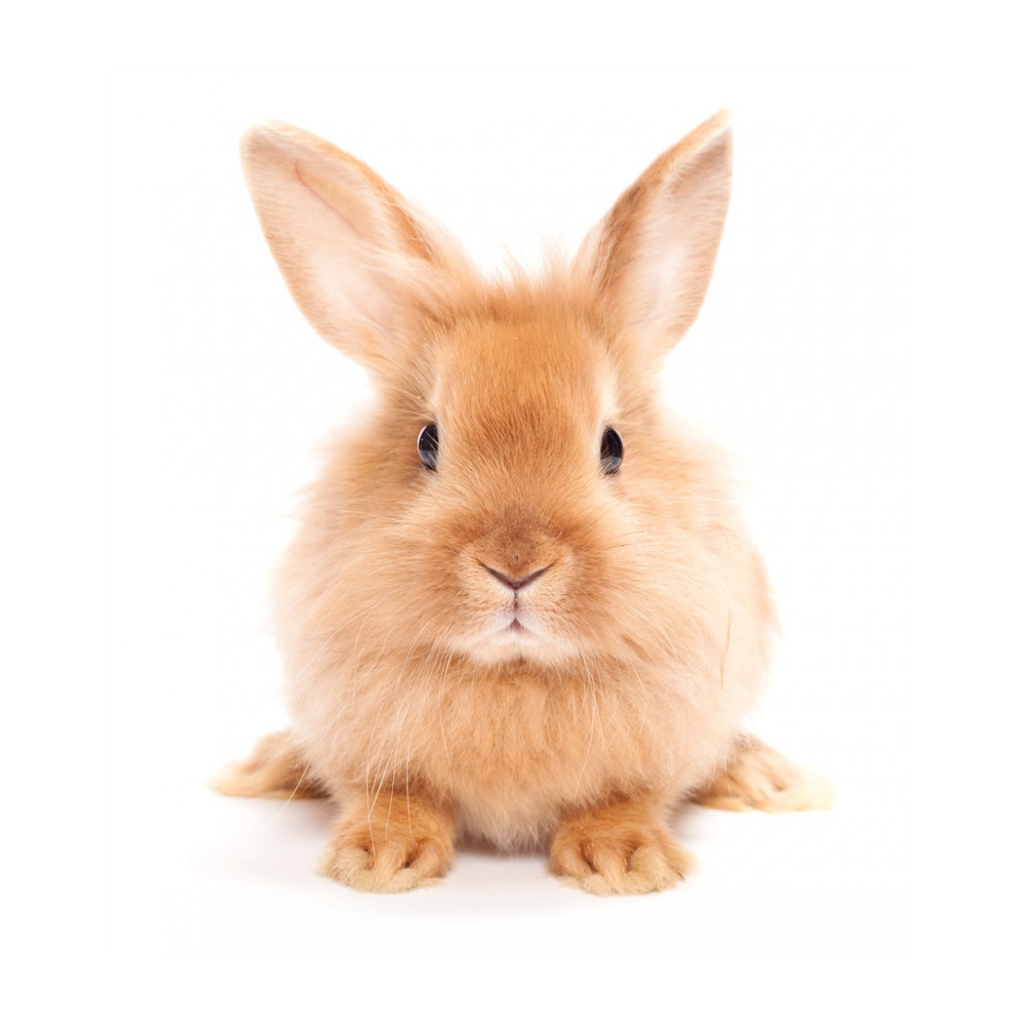
\includegraphics[width=0.25\linewidth]{image.png}
\end{figure}
\subsection*{} \href{https://problems.ru/articles/216.php}{Статья о принципе Дирихле} 
\subsection*{Принцип Дирихле} 
Наиболее часто принцип Дирихле формулируется в следующей форме: \textbf{Если $n + 1$ кролик помещен в $n$ клеток, то хотя бы в одной из клеток находятся не менее двух кроликов}. Другими словами, нельзя посадить $n + 1$ кролика в $n$ клеток, чтобы в каждой клетке было не больше 1 кролика. \\ Главная задача - найти кроликов и клетки, тогда мы получим неконструктивное доказательство (то есть мы точно знаем, что в какой-то клетке кроликов больше, но в какой конкретно - нам не важно)
\subsection*{Обобщённый принцип Дирихле} Если есть n клеток и \textbf{больше} nk кроликов, то хотя бы в одной клетке больше k кроликов.

\subsection*{Упражнения}
\begin{enumerate}
    \item Имеется 25 конфет 3 сортов. Верно ли, что не менее 9 из них будут какого-то одного сорта?
    \item Обязательно ли среди двадцати пяти "медных" монет (т.е. монет достоинством 1, 2, 3, 5 коп.) найдётся семь монет одинакового достоинства?
    \item Докажите, что из любых 12 натуральных чисел можно выбрать два, разность которых делится на 11. 
    \item Имеется 101 пуговица одного из 11 цветов. Докажите, что либо среди этих пуговиц найдутся 11 пуговиц одного цвета, либо 11 пуговиц разных цветов.
    \item Докажите, что из любых семи натуральных чисел (не обязательно идущих подряд) можно выбрать три числа, сумма которых делится на 3.
    \item Доказать, что если 21 человек собрали 200 орехов, то есть два человека, собравшие поровну орехов.
\end{enumerate}

\subsection*{Задачи посложнее}
\begin{enumerate}
    \item \begin{enumerate}
        \item По кругу в произвольном порядке расставлены числа от 0 до 23, докажите, что сумма некоторых трёх подрядыдущих чисел не меньше 36.
        \item По кругу в произвольном порядке расставлены числа от 1 до 23, докажите, что сумма некоторых трёх подрядыдущих чисел не меньше 36.
    \end{enumerate}
    \item Можно ли в клетках квадратной таблицы $5 \cdot 5$ расставить числа 0, +1, –1 так, чтобы все суммы в каждом столбце, в каждой строке и на каждой из двух диагоналей были различны? 
    \item Все клетки бесконечной клетчатой доски покрашены в белый или чёрный цвет. Известно, что в каждом квадрате $3 \cdot 3$ не более 5 белых клеток. Докажите, что в каком-нибудь квадрате $4 \cdot 4$ не блее 8 белых клеток. (Подсказка: можно рассмотреть какую-нибудь удобную ограниченную фигуру)
    \item Имеется  2k + 1  карточек, занумерованных числами от 1 до  2k + 1.  Какое наибольшее число карточек можно выбрать так, чтобы ни один из извлечённых номеров не был равен сумме двух других извлечённых номеров?
\end{enumerate}

\end{document}
